\documentclass[a4paper,oneside]{book}

%%% INICIO DEL PREÁMBULO %%%

\usepackage[utf8]{inputenc}
\usepackage[greek,spanish,es-tabla,es-nodecimaldot,es-noindentfirst]{babel}
\usepackage{babelbib}
\usepackage{nccmath}
\usepackage{amsthm}
\usepackage{lipsum}
\usepackage{tcolorbox}
\usepackage[thicklines]{cancel}
\usepackage{mathtools}
\usepackage{amssymb}
\usepackage{amsmath}
\usepackage{caption}
\usepackage{subcaption}
\usepackage{color}
\usepackage{verbatim}
\usepackage{enumerate}
\usepackage{geometry}
\geometry{a4paper,left=35mm,right=35mm,top=15mm,bottom=15mm}
\usepackage{isotope}
\usepackage{maybemath}
\usepackage{upgreek}
\usepackage{wasysym}
\usepackage[italic]{hepparticles}
\usepackage{subdepth}
\usepackage{siunitx}
\sisetup{
	mode 			= text,
	parse-units 	= false
}
\usepackage{physics}
\usepackage{braket}
\usepackage{tensor}
\usepackage{chemformula}
\usepackage{tikz}
\usepackage{url}
\usepackage{listings}
\usepackage{multirow}
\usepackage{multicol}
\usepackage[colorlinks=true]{hyperref}
\hypersetup{
	citecolor = blue,
	linkcolor = blue,
	urlcolor = blue,
	pdfauthor = {Javier Rodrigo López}
}
\usepackage{eso-pic}

% tikz
\usepackage{tikz} \usetikzlibrary{fit,babel,shapes,arrows,patterns,positioning,calc,decorations.pathmorphing,decorations.markings}
\tikzstyle{block} = [draw, fill=white, rectangle,
minimum height=3em, minimum width=6em]
\tikzstyle{sum} = [draw, fill=white, circle, node distance=1cm]
\tikzstyle{input} = [coordinate]
\tikzstyle{output} = [coordinate]
\tikzstyle{pinstyle} = [pin edge={to-,thin,black}]
\tikzset{
	block/.style = {draw, fill=white, rectangle, minimum height=3em, minimum width=3em},
	tmp/.style  = {coordinate},
	sum/.style= {draw, fill=white, circle, node distance=1cm},
	input/.style = {coordinate},
	output/.style= {coordinate},
	pinstyle/.style = {pin edge={to-,thin,black}}
}

\usepackage[oldvoltagedirection]{circuitikz}
\usepackage{pdflscape}

% Títulos
\usepackage{titlesec}
\titleformat{\section}{\normalfont\Large\bfseries}{\thesection}{1em}{}[{\titlerule[0.8pt]}]
% \renewcommand{\thesubsection}{\arabic{chapter}.\arabic{section}.\Alph{subsection}}
\titleformat{\subsubsection}{\normalfont\normalsize\bfseries}{\thesubsubsection}{1em}{}[{\titlerule[0.05pt]}]
\titlespacing{\section}{0pt}{2\parskip}{\parskip}
\titlespacing{\subsection}{0pt}{\parskip}{0pt}
\titlespacing{\subsubsection}{0pt}{\parskip}{0pt}

% Numeración de secciones
\setcounter{tocdepth}{2}
\setcounter{secnumdepth}{2}

% Figuras y descripciones
\renewcommand{\thefigure}{\arabic{figure}}
\renewcommand{\thesubfigure}{\Alph{subfigure}}
\captionsetup[figure]{labelfont={bf},name={Figura},labelsep=period}
\numberwithin{figure}{chapter}
\numberwithin{equation}{chapter}

% Enumerations
\newcounter{myenumi}
\renewcommand{\themyenumi}{\alph{myenumi})}
\newenvironment{myenumerate}{\setlength{\parindent}{0pt}\setcounter{myenumi}{0}\renewcommand{\item}{\par\refstepcounter{myenumi}\makebox[1.3em][l]{\themyenumi}}}{\par\bigskip\noindent\ignorespacesafterend}

% Own environments
\newenvironment{nota}{\underline{\textbf{NOTA:}} }{}
\newenvironment{caja}{\begin{tcolorbox}[colback = white, sharp corners, boxrule = 1 pt]}{\end{tcolorbox}}
\newtheorem*{conclusion}{Conclusión}
\newtheorem{teorema}{Teorema}
\newtheorem{definicion}{Definición}

% Para una bonita portada
\usepackage{wallpaper}
\usepackage{titling}
\usepackage{fancyhdr}
\pagestyle{fancy}
\setlength{\droptitle}{-10cm}
\renewcommand{\chaptermark}[1]{%
	\markboth{#1}{}}
\renewcommand{\sectionmark}[1]{%
	\markright{}}
\fancyhf{}
\fancyhead[LE,RO]{\bfseries\thepage} \fancyhead[LO]{\bfseries\rightmark} \fancyhead[RE]{\bfseries\leftmark} \renewcommand{\headrulewidth}{0pt} \renewcommand{\footrulewidth}{0pt} \addtolength{\headheight}{15pt}
\fancypagestyle{plain}{%
	\fancyhead{}
	\renewcommand{\headrulewidth}{0pt}
}

% Organización del texto
\newcommand{\formula}[1]{\vspace{13 pt}\noindent \textbf{\underline{#1}}}
\newcommand{\subtext}[1]{_{\text{#1}}}

% Unidades y utilidades varias
\renewcommand{\S}{\operatorname{S}}
\newcommand{\dB}{\operatorname{dB}}
\newcommand{\dBW}{\operatorname{dBW}}
\newcommand{\dBm}{\operatorname{dBm}}
\newcommand{\Hz}{\operatorname{Hz}}
\newcommand{\s}{\operatorname{s}}
\newcommand{\A}{\operatorname{A}}
\newcommand{\V}{\operatorname{V}}
\newcommand{\ohm}{\,\Omega}
\newcommand{\Pa}{\operatorname{Pa}}
\newcommand{\W}{\operatorname{W}}
\newcommand{\I}{\operatorname{I}}
\newcommand{\C}{\operatorname{C}}
\newcommand{\K}{\operatorname{K}}
\newcommand{\m}{\operatorname{m}}
\newcommand{\mm}{\operatorname{mm}}
\newcommand{\rad}{\operatorname{rad}}
\newcommand{\mol}{\operatorname{mol}}
\newcommand{\J}{\operatorname{J}}
\newcommand{\kg}{\operatorname{kg}}
\newcommand{\incremento}{\Delta}
\newcommand{\psus}{\, \ldots \,}
\newcommand{\mcm}{\operatorname{mcm}}
\newcommand{\MCD}{\operatorname{MCD}}
\renewcommand{\sin}{\sen}
\renewcommand{\arcsin}{\arcsen}
\renewcommand{\arctan}{\arctg}
\renewcommand{\min}{\operatorname{mín}}

\DeclarePairedDelimiter\evaluat{.}{\rvert}

% Vectores
\usepackage[c]{esvect}
\renewcommand{\vec}[1]{\vv{{#1}}}
\newcommand{\proy}[2]{\operatorname{proy}_{\vec{#2}}\vec{#1}}
\newcommand{\antiparallel}{\downharpoonleft \! \upharpoonright}
\newcommand{\parallelvec}{\upharpoonleft \! \upharpoonright}

% Espaciado
\usepackage{enumitem}
\setlist{before={\parskip=3pt}, after=\vspace{\baselineskip}}
\setlength{\parindent}{0pt}
\setlength{\parskip}{0.5em}

% Estadística
\DeclareMathOperator{\Var}{Var}
\DeclareMathOperator{\Cov}{Cov}
\renewcommand{\var}{\sigma ^2}
\DeclareMathOperator{\B}{B}
\DeclareMathOperator{\BN}{BN}
\DeclareMathOperator{\Geo}{Geo}
\DeclareMathOperator{\Poisson}{Poisson}
\DeclareMathOperator{\U}{U}
\DeclareMathOperator{\Exp}{Exp}
\DeclareMathOperator{\N}{N}
\DeclareMathOperator{\Mult}{Mult}
\newcommand{\TF}[1]{\mathrm{TF} \left\lbrace \left. #1 \right\rbrace \right.}
\newcommand{\probCond}[2]{P \left( #1 \: \middle\vert\:  #2 \right) }

% Electromagnetismo y Ondas
\newcommand{\errorGrave}{\textbf{FG!!!}}
\newcommand{\mas}{M.A.S.}
\newcommand{\mcu}{M.C.U.}
\newcommand{\ed}{E.D.}
\newcommand{\edmas}{E.D. del M.A.S.}
\usepackage{esint}

% Señales y Sistemas
\renewcommand{\H}{H}

% Circled number
\newcommand{\circledNumber}[1]{\raisebox{.9pt}{\textcircled{\raisebox{-.9pt}{#1}}}}

% Footnotes
% \renewcommand{\thefootnote}{\fnsymbol{footnote}}

% Ejemplo
\newcounter{elejemplo}
\newcommand{\ejemplo}[2]{
	\refstepcounter{elejemplo}
	\begin{center}
		\fbox{\begin{minipage}{0.85\linewidth}
			\textbf{Ejemplo \arabic{elejemplo}.} #1
			\begin{center}
				\underline{\textbf{Solución}}
			\end{center}
			#2
		\end{minipage}}
	\end{center}
}

% Repeticiones
\usepackage{forloop}
\newcommand{\repvec}[3]{
	\foreach \uwu in {1,...,#2}
		{\vec{#1}_{\uwu} ,}
	\, \ldots \, , \vec{#1}_{#3}
}
\newcommand{\rep}[3]{
	\foreach \uwu in {1,...,#2}
		{#1_{\uwu} ,}
	\, \ldots \, , #1_{#3}
}
\newcommand{\repinf}[3]{
	\foreach \uwu in {#2,...,#3}
		{#1_{\uwu} ,}
	\, \ldots
}

%%% FIN DEL PREÁMBULO %%% % Se incluye el preámbulo

% Título y portada
\title{\Huge Procesado Digital de la Señal\\\vspace*{5pt}
\Large Apuntes de clase}
\author{Javier Rodrigo López \thanks{Correo electrónico: \href{mailto:javiolonchelo@gmail.com}{\texttt{javiolonchelo@gmail.com}}}} 
\date{\today}

%%% INICIO DEL DOCUMENTO %%%
\begin{document}

\setlength{\wpYoffset}{-0.5cm}
\setlength{\droptitle}{-10cm}
\ThisCenterWallPaper{0.7}{./Imágenes/Velazquez.jpg}
\maketitle

\titleformat{\chapter}[block]
{\normalfont\Huge\bfseries}{\huge{TEMA \thechapter.}\\ }{1em}{}

% Marca de agua
\AddToShipoutPictureFG{
	\begin{tikzpicture}[overlay,remember picture]
		\path (current page.south west) -- (current page.north east)
		node[midway,scale=8,color=lightgray,sloped,opacity=0.05] {Javier Rodrigo López};
	\end{tikzpicture}
}

% Logotipos UPM y ETSIST
\begin{figure}[t!]
	\centering
	\begin{subfigure}[b]{0.65\linewidth}
		
\includegraphics[width=\linewidth]{../../Archivos comunes/upm_logo.png}
	\end{subfigure}
	\begin{subfigure}[b]{0.25\linewidth}
		
\includegraphics[width=\linewidth]{../../Archivos comunes/etsist_logo.png}
	\end{subfigure}
\end{figure}

% Introducción
\newpage
\phantomsection
\addcontentsline{toc}{section}{Introducción}
\section*{Introducción}
Imagen de la portada: \textsl{La fragua de Vulcano}, por Diego Velázquez.

Las clases en las que se basan estos apuntes fueron impartidas por:
\begin{itemize}
	\item  \href{mailto:cesar.diazm@upm.es}{César Díaz Martín}
	\item \href{mailto:eduardo.latorre.iglesias@upm.es}{Eduardo Latorre Iglesias}
\end{itemize}

\newpage

% Índice (TOC)
\setlength{\parskip}{0em}
\tableofcontents
\setlength{\parskip}{0.5em}

%%% INICIO DE LOS APUNTES %%%

\chapter{Transformada de Fourier y Muestreo}

\section{Introducción a la Transformada de Fourier}

\section{Series de Fourier de señales periódicas}

\subsection{Fenómeno de Gibbs}

En una señal que necesite infinitos coeficientes de Fourier para ser representada de forma exacta, al coger solo un conjunto de los coeficientes se produce un ``rizado'' en ciertos puntos de la señal, con amplitud independiente del número de coeficientes escogidos. Este suceso es lo que se conoce como \textbf{fenómeno de Gibbs}.

\section{Transformada de Fourier para señales no periódicas}

\subsection{Propiedades de la transformada de Fourier}

\section{Transformada de Fourier de señales periódicas}

\chapter{Procesado digital de señales analógicas}

\section{Tipos de señal} \vspace{\parskip}

\subsection{Señales continuas}

En una señal periódica, podemos obtener el \textbf{periodo} como el mínimo común múltiplo de los periodos de sus componentes. Un ejemplo:

\[ x(t) = 3 \sen \left( 5\pi t + \frac{\pi}{4} \right) + \cos \left( 10\pi t \right)\, ;\qquad \omega_1 = 5\pi \, , \quad \omega_2 = 10\pi \]
\[ T = \mcm \left( \frac{2\pi}{\omega_1} \, , \frac{2\pi}{\omega_2} \right) = \mcm \left( \frac{2\pi}{5\pi} \, , \frac{2\pi}{10\pi} \right) = \mcm \left( \frac{2}{5} \, , \frac{1}{5} \right) = \frac{1}{5} \mcm \left( 2 \, , 1 \right) = \boxed{\frac{2}{5} \, \unit{\s}}\]

\subsection{Señales discretas}

El \textbf{periodo} de una señal discreta se obtiene de forma similar a las señales continuas. Sin embargo, cuando el resultado es una fracción el periodo se calcula como el numerador de dicha fracción.

Siguiendo con el ejemplo anterior, a partir de la última fracción obtenida:
\[ \frac{N}{m} = \frac{2}{5} \quad \Longrightarrow \quad \boxed{N = 2} \]

\section{Filtros}

Un \textbf{filtro} es cualquier sistema que modifica la forma de la señal, tanto en su amplitud como en su fase, del modo deseado. Los catalogamos como \textbf{FIR}\footnote{FIR $\equiv$ \textit{Finite Impulse Response.}} o \textbf{IIR}\footnote{IIR $\equiv$ \textit{Infinite Impulse Response.}}, en función de su respuesta al impulso.

Hablaremos de ellos con profundidad en el Tema \ref{temaDeFiltros}.

\section{Estructura de un sistema PDS}

A continuación, se encuentra representado el esquema general de un sistema PDS:

\begin{figure}[ht]
	\centering
	\caption{Esquema de un sistema PDS} \label{fig:esquema_PDS}
	\begin{tikzpicture}[auto,>=latex']
		\node [input, name=input] (input) {};
		\node [block, below of=input, node distance=0cm] (A) {$
		\begin{matrix}
			\text{Filtro}\\
			\text{anti-aliasing}
		\end{matrix}$};
		\node [block, right of=A, node distance=2.5cm] (B) {ADC};
		\node [block, right of=B, node distance=2.5cm] (C) {$
		\begin{matrix}
			\text{Proceso}\\
			\text{digital}
		\end{matrix}$};
		\node [block, right of=C, node distance=2.5cm] (D) {DAC};
		\node [block, right of=D, node distance=2.5cm] (E) {$
		\begin{matrix}
			\text{Filtro de}\\
			\text{salida}
		\end{matrix}$};

		\draw [-angle 90] (-2,0) --  node{$x(t)$} (A);
		\draw [-angle 90] (A) --  node{$x'(t)$} (B);
		\draw [-angle 90] (B) --  node{$x[n]$} (C);
		\draw [-angle 90] (C) --  node{$y[n]$} (D);
		\draw [-angle 90] (D) --  node{$y'(t)$} (E);
		\draw [-angle 90] (E) --  node{$y(t)$} ++(2,0);
	\end{tikzpicture}
\end{figure}

\newpage

\section{Muestreo}

El muestreo es la recogida de muestras temporalmente equiespaciadas de una señal analógica para conformar una señal discreta.

\subsection{Teorema de Nyquist}

Para realizar el muestreo de una señal sin que se produzca aliasing\footnote{El \textit{aliasing} es el solapamiento espectral producido por el submuestreo.} debemos asegurar que se cumple el \textbf{Teorema de Nyquist}. Este afirma que la frecuencia de muestreo debe ser, al menos, el doble de la frecuencia máxima de la señal a muestrear\footnote{El subíndice ``s'' viene de \textit{sampling} (en inglés, muestreo). El subíndice ``m'' viene de \textit{max}.}:
\[ w_s \geq 2w_m \]

Un ejemplo curioso es el caso de los CDs de audio. Como los humanos somos capaces de escuchar hasta \SI{20}{\kHz} (aproximadamente), los CDs tienen una frecuencia de muestreo un poquito mayor al doble de esta: \SI{44.1}{\kHz}.

\subsection{Evitar solapamiento}

Sabiendo que si no se cumple el teorema de Nyquis (debido al submuestreo) podemos llegar a experimentar solapamiento espectral, tenemos dos alternativas para enfrentarnos a este problema.
\begin{itemize}
	\item \textbf{Aumentar la frecuencia de muestreo}. Es la opción más directa y sencilla. Sin embargo, muchas veces los sistemas que usemos serán limitados. Esta no es una opción que siempre podamos usar.
	\item Utilizar un \textbf{filtro anti-solapamiento}. El uso de un filtro paso bajo con frecuencia de corte $\omega_c = \omega_s/2$ asegura el procesado de la señal limpia. En la práctica, la pérdida de señal es menos perjudicial que los efectos del aliasing.
\end{itemize}

\subsection{Teorema del muestreo discreto}

Para evitar el solapamiento espectral, se debe cumplir: \[ Q \leq \frac{\pi}{\Omega_m}\]
Donde $Q$ es el número de réplicas que caben en el espectro de la señal a muestrear. En otras palabras, $Q$ es el \textbf{orden de diezmado}.


\subsection{Teorema de la interpolación}

Sea $x[n]$ una señal discreta a la que queremos realizar interpolación de orden $P$, la señal interpolada resultante tendrá la forma:
\[ x_P[n] = \left\lbrace 
\begin{matrix*}[l]
	x \left[ \frac{n}{P} \right] & \text{si } n = \dot{P}\\[5pt]
	0 & \text{resto}
\end{matrix*} \right.\]

Lo que se traduce en posicionar $P-1$ ceros entre cada muestra de la señal original.

Es importante saber que una \underline{expansión} en el tiempo conlleva una \underline{compresión} en frecuencia.

\section{Sistemas equivalentes. C/D y D/C}

Para trabajar con sistemas continuos y discretos, se deben establecer unos criterios de equivalencia. En resumidas cuentas, los sistemas equivalentes se basan en la siguiente característica:

\[ H_D \left( e^{j\omega } \right) = \biggl. H_C \left( j\omega \right)  \biggr\vert _{\omega = \frac{\Omega}{T_s}} \]

\begin{itemize}
	\item La propiedad de \textbf{invarianza temporal} surge de la relación entre el tiempo continuo y el tiempo discreto: $t = nT_s $
	\item Cuando introducimos una señal continua $x(t)$ en un conversor C/D, la señal discreta que tenemos a la salida resulta escalada en un factor $\frac{1}{T_s}$ con respecto a $x(t)$. Si te surgen dudas, mira en la tabla de transformadas y propiedades de la DFT.
\end{itemize}

\ejemplo
{
	Obtenga el sistema discreto que permite implementar el siguiente sistema LTI continuo:
	\[ H_C \left( j\omega \right) = \left\lbrace
		\begin{matrix*}[l]
			1	&, \abs{\omega }<\omega _c\\
			0	&, \text{ resto}
		\end{matrix*} \right. \]
}
{
	\begin{align*}
		H_D \left( e^{j\omega} \right) & = \biggl. H_C \left( j\omega \right) \biggr\vert_{\omega = \frac{\Omega}{T_s}} = H_C \left( j \frac{\Omega}{T_s} \right) \quad , \abs{\Omega}<\pi \\[10pt]
		H_D \left( e^{j\omega} \right) & = \left\lbrace
		\begin{matrix*}[l]
			1 & , \abs{\frac{\Omega}{T_s} }<\omega _c\\
			0 & , \text{ resto}
		\end{matrix*} \right. = \boxed{\left\lbrace
		\begin{matrix*}[l]
			1 & , \abs{\Omega}<\omega _cT_s<\pi\\
			0 & , \text{ resto}
		\end{matrix*} \right.}
	\end{align*}
Siempre y cuando se cumpla que $\omega_s\geq 2\omega_c$, podré emular en todo el rango de frecuencias de interés $H_c \left( j\omega \right)$
}

\section{Cambio de velocidad de muestreo}

El cambio de velocidad de muestreo (también denominado procesado multitasa) pretende obtener a partir de una señal discreta otra señal discreta con diferente frecuencia de muestreo.

\subsection{Expansor y Compresor}

Un \textbf{expansor} es un elemento que realiza la interpolación. Un \textbf{compresor} es un elemento que realiza el diezmado. Sin embargo, este último lo consigue en dos pasos:
\begin{itemize}
	\item Muestreo con $T_s = Q$.
	\item Supresión de $Q - 1$ ceros (lo opuesto a la interpolación).
\end{itemize}

En un sistema real, lo preferible es hacer uso del expansor antes que el compresor.

\section{Aspectos prácticos}

El proceso de muestreo y reconstrucción de una señal nunca es ideal. Se producirán errores, que pueden ser minimizados en función de los parámetros que escojamos en cada proceso.

El \textbf{ADC} agrupa el conjunto de operaciones que nos permite convertir una señal de entrada continua en una señal analógica.

\begin{figure}[ht]
	\centering
	\caption{Etapa de entrada ADC} \label{fig:esquema_ADC}
	\begin{tikzpicture}[auto,>=latex']
		\node [input, name=input] (input) {};
		\node [block, below of=input, node distance=0cm] (A) {$
		\begin{matrix}
			\text{Filtro}\\
			\text{anti-aliasing}
		\end{matrix}$};
		\node [block, right of=A, node distance=2.5cm] (B) {$
		\begin{matrix}
			\text{Sampler}\\
			\text{\& Hold}
		\end{matrix}$};
		\node [block, right of=B, node distance=2.5cm] (C) {Cuantificador};
		\node [block, right of=C, node distance=2.5cm] (D) {Codificador};

		\draw [color=red,thick, dashed](1.5,-1) rectangle (8.75,1);
		\node[text width=3cm] at (9.25,1.25) {\textbf{ADC}};

		\draw [-angle 90] (-2.5,0) --  node{$x(t)$} (A);
		\draw [-angle 90] (A) --  node{} (B);
		\draw [-angle 90] (B) --  node{} (C);
		\draw [-angle 90] (C) --  node{} (D);
		\draw [-angle 90] (D) --  node{$x[n]$} ++(2.5,0);
	\end{tikzpicture}
\end{figure}

\subsection{Filtro antialiasing}

Para evitar el aliasing, debemos usar un filtro paso bajo que, idealmente, tendría la siguiente forma:
\[ H_{aa}(j\omega ) = \left\lbrace 
\begin{matrix*}[l]
	1 \, , & \abs{\omega}<\omega_c \leq \frac{\omega_s}{2}\\ 
	0 \, , & \abs{\omega} > \omega_c
\end{matrix*} \right. \] 

Sin embargo, en la realidad es muy complicado implementar un filtro de este estilo. La solución alternativa es el \textbf{sobremuestreo}. Si conseguimos $\omega_s \gg 2 \omega_m$, podemos implementar un filtro que no altere demasiado la información a filtrar.
	
Se define entonces la \textbf{tasa de sobremuestreo} $R$ como:
\[ R = \frac{\omega_s}{2\omega_m} \]

\subsection{Sampler \& Hold}

Este circuito sirve para seleccionar ciertas muestras equiespaciadas en el tiempo de una señal continua dada y mantener su valor hasta obtener la siguiente muestra.

\begin{figure}[htp] \label{fig:samplerAndHold}
	\centering
	\caption{Ejemplo de señal procesada por un circuito Sampler \& Hold}
	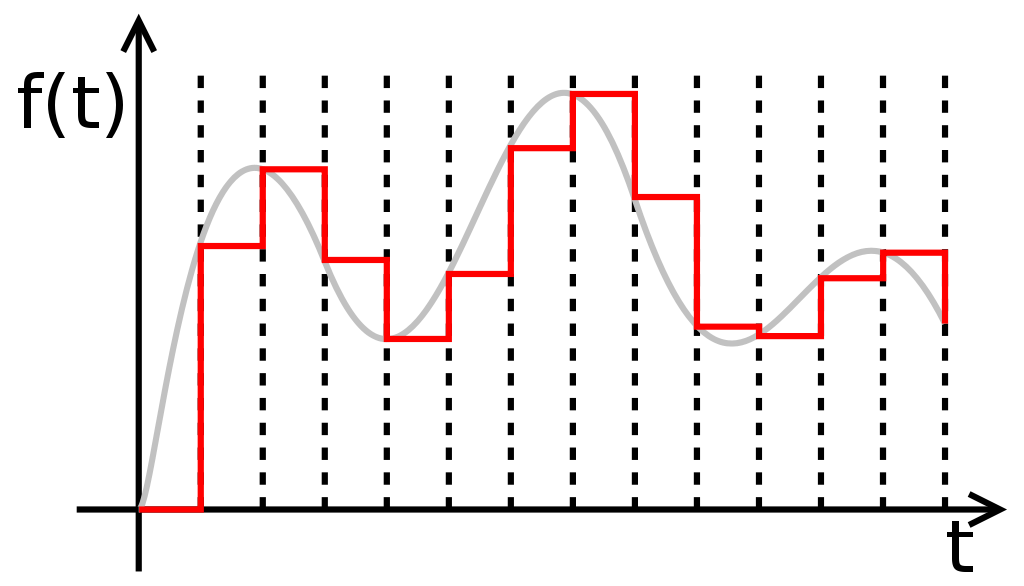
\includegraphics[width=0.8\linewidth]{Imágenes/SamplerAndHold.png}
\end{figure}

\subsection{Cuantificador y Codificador}

Un cuantificador es una etapa que asigna a cada valor leído en su entrada un valor binario de $n$ bits, de modo que puede leer $2^n$ valores diferentes (que se corresponden con los escalones proporcionados a la salida del Sampler \& Hold).

Puedes ver un ejemplo del procesado de una señal a través de un cuantificador uniforme en la \autoref{fig:cuantificadorUniforme}.

\begin{figure}[htp]
	\centering
	\caption{Ejemplo de señal procesada en un cuantificador uniforme.}\label{fig:cuantificadorUniforme}
	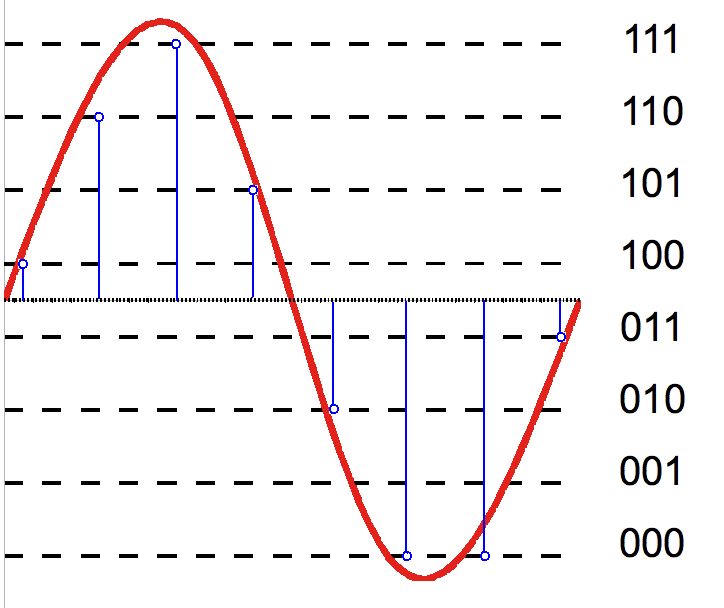
\includegraphics[width=0.6\linewidth]{Imágenes/Quantification.png}
\end{figure}

\subsubsection{Error de Cuantificación}

Para tratar con el ruido en estos sistemas, vamos a suponer siguie el modelo estadístico del ruido:
\begin{itemize}
	\item El error es un proceso estocástico estacionario.
	\item La secuencia $e[n]$ está incorrelada con $x[n]$.
	\item El error es un proceso de ruido blanco.
	\item La función densidad de probabilidad (FDP) del error es uniforme entre $-\Delta / 2$ y $+\Delta / 2$.
\end{itemize}

Estas suposiciones se cumplen si la señal a tratar es complicada, fluctuando de manera rápida e impredecible, y  si el escalón de cuantificación es suficientemente pequeño.

Podemos calcular varias cosas a partir de esto.
\begin{itemize}
	\item \textbf{Potencia del error.} \[ \sigma_e^2 = \frac{\Delta ^2}{12} = \frac{x_m^2}{12 \cdot 2^{2b}} \]
	\item \textbf{Relación señal a ruido (SNR)}
	\begin{align*}
		\textrm{SNR}(\unit{\dB}) &= 10 \log \left( \frac{\sigma_x^2}{\sigma_e^2} \right) \\ 
		&= 10 \log \left( 12 \right) + 10 \log \left( 2^{2b} \right) + 10 \log \left( \frac{\sigma_x^2}{x_m^2} \right) \\
		&= \boxed{10.79} + \boxed{6.02 \cdot b} + \boxed{20 \log \left( \frac{x_m}{\sigma_x} \right) }
	\end{align*}
\end{itemize}

\chapter{Transformada Discreta de Fourier: DFT}

\section{Definición, cálculo, relaciones y propiedades}

\subsubsection{Ecuación de análisis}
	
\[ X_K = \sum_{n=0}^{M-1}\tilde{x}[n]e^{-jk \frac{2\pi}{M}K n} \, , \quad 
\begin{matrix*}[l]
	K = 0, 1, \ldots , M-1 \\[5pt]
	\Omega = 0, \frac{2\pi}{M}, \frac{4\pi}{M}, \ldots , 2\pi - \frac{2\pi}{M}
\end{matrix*}\]
	
\subsubsection{Ecuación de síntesis}
	
\[ \tilde{x}[n] = \frac{1}{M} \sum_{n=0}^{M-1}X_Ke^{j \frac{2\pi}{M}Kn}\]


\subsection{Conversión a secuencia discreta}

La conversión de la DFT de una señal a una secuencia discreta se realiza con la simple relación $\Omega = \omega T_s$, adaptándola según necesitemos. A continuación, la forma de llevarlo a la práctica:

\[ X \left( \omega \right) = \biggl. X \left( \Omega \right)  \biggr\vert _{\Omega = \omega T_s} \qquad \qquad X \left( \Omega \right) = \biggl. X \left( \omega \right)  \biggr\vert _{\omega = \frac{\Omega}{T_s}} \]

La TF de una señal discreta es una señal continua periódica. Sin embargo, para operar con las frecuencias en el terreno digital es mucho más cómodo realizar un muestreo de la misma.

La \textbf{DFT} es simplemente un muestreo realizado entre $0$ y $2\pi$ de $M$ muestras, siendo $M$ el orden de la DFT\footnote{Normalmente se denota como $\DFT^M$ para indicar directamente que la DFT es de orden $M$.}.

Este muestreo se realiza de una forma completamente diferente a como lo hacíamos en un ADC. Si recuerdas, la TF surgía como una serie de Fourier de una señal cuando su periodo tendía a infinito. De forma análoga, podemos obtener realizar el desarrollo en series de Fourier de una señal no periódica si forzamos su repetición, de modo que su nuevo periodo sea $N = M$.

\[ a_k = \biggl. \frac{1}{M} X(\Omega ) \biggr\vert _{\Omega = k \frac{2\pi}{M}}\]

Suponemos que la señal $x[n]$ tiene $L$ muestras, podemos tener dos situaciones:
\begin{multicols}{2}
	\begin{itemize}
		\item \textbf{Sobremuestreo:} $\boxed{M\geq L}$
		\item \textbf{Submuetreo:} $\boxed{M<L}$
	\end{itemize}
\end{multicols}

Cuando se realiza un submuestreo, no se puede recuperar la señal original una vez hayamos calculado la DFT, cosa que no sucedería si se realizara un sobremuestreo.

Sin embargo, en ambas situaciones se puede realizar la DFT. Simplemente debemos saber lo que conlleva.

\subsection{Orden mínimo de la DFT}

Cuando una señal que es combinación lineal de funciones armónicas de diferentes frecuencias, se puede calcular el orden mínimo necesario de la DFT para representar dichas frecuencias como:
\[ \Omega_i = \frac{2\pi k_i}{M_i} \qquad \Longrightarrow \qquad \boxed{\frac{k_i}{M_i} = \frac{\Omega _i}{2\pi}} \]

\subsection{Cálculo matricial}

También es posible obtener la DFT realizando el \textbf{cálculo matricial de la DFT}:

\[ \left( 
\begin{matrix}
	X[0]\\
	X[1]\\
	\vdots \\
	X[F]\\
\end{matrix} \right)
= \left(
\begin{matrix}
	W^{0 \cdot 0} & W^{0 \cdot 1} & \cdots & W^{0 \cdot F}\\
	W^{1 \cdot 0} & W^{1 \cdot 1} & \cdots & W^{1 \cdot F}\\
	\vdots & \vdots & \ddots & \vdots \\
	W^{F \cdot 0} & W^{F \cdot 1} & \cdots & W^{F \cdot F}\\
\end{matrix} \right)
\left( \begin{matrix}
	\tilde{x}[0]\\
	\tilde{x}[1]\\
	\vdots\\
	\tilde{x}[F]\\
\end{matrix} \right)
\qquad \quad 
\begin{matrix*}[l]
	W^{K \cdot n} = e^{-j \frac{2\pi}{M}Kn}\\[5pt]
	F = M - 1
\end{matrix*}
\]

De forma análoga, podemos realizar el \textbf{cálculo matricial de la DFT inversa}:

\[ \left( \begin{matrix}
	\tilde{x}[0]\\
	\tilde{x}[1]\\
	\vdots\\
	\tilde{x}[F]\\
\end{matrix} \right)
= \left(
\begin{matrix}
	v^{0 \cdot 0} & v^{0 \cdot 1} & \cdots & v^{0 \cdot F}\\
	v^{1 \cdot 0} & v^{1 \cdot 1} & \cdots & v^{1 \cdot F}\\
	\vdots & \vdots & \ddots & \vdots \\
	v^{F \cdot 0} & v^{F \cdot 1} & \cdots & v^{F \cdot F}\\
\end{matrix} \right)
\left( 
\begin{matrix}
	X[0]\\
	X[1]\\
	\vdots \\
	X[F]\\
\end{matrix} \right)
\qquad \quad 
\begin{matrix*}[l]
	v^{K \cdot n} = \frac{1}{M} e^{j \frac{2\pi}{M}Kn}\\[5pt]
	F = M - 1
\end{matrix*}
\]

\section{Introducción al análisis espectral mediante la DFT}

\subsection{Enventanado}

En los sistemas reales, no podemos coger muestras infinitas de una señal. Al acto de escoger $L$ muestras de la señal original se le denomina \textbf{enventanado}. 

Se pueden modificar los parámetros según lo que se quiera conseguir. Algunas modificaciones que se pueden hacer:
\begin{itemize}
	\item \textbf{Ancho del lóbulo principal.} Solo depende de $L$. \[ \uparrow L \quad \downarrow W \quad \uparrow \textrm{Tiempo de adquisición} \]
	\item \textbf{Ancho de los lóbulos secundarios.} Corresponde a las \textbf{fugas espectrales}, energía que aparece en frecuencias no deseadas. Solo depende del \textbf{tipo de ventana}.
\end{itemize}

A efectos prácticos, es como multiplicar la señal por una ventana rectangular de longitud $L$. Vamos a ver qué tipos de ventana podemos usar y qué efectos tienen en la DFT.

\newpage

\begin{multicols}{2}
	\subsubsection{Ventana rectangular}\vspace{\parskip}
	\begin{itemize}
		\item Lóbulo lateral a \textbf{13 dB} por debajo del lóbulo principal.
		\item La anchura del lóbulo principal se reduce a menuda que se aumenta la longitud de la ventana.
	\end{itemize}
	\[ w[n] = \left\lbrace 
	\begin{matrix*}[l]
		1 & -M\leq n \leq M\\
		0 & \textrm{resto}
	\end{matrix*} \right. \]

	\subsubsection{Ventana de Hanning}\vspace{\parskip}
	\begin{itemize}
		\item Lóbulo lateral a \textbf{31 dB} por debajo del lóbulo principal.
		\item La anchura del lóbulo principal es aproximadamente el doble que en la ventana rectangular, y se reduce según aumenta $L$.
	\end{itemize}
	\[ w[n] = \left\lbrace
	\begin{matrix*}[l]
		\displaystyle{\frac{1}{2} + \frac{1}{2}\cos \left( \frac{\pi}{M+1}n \right)} & -M\leq n \leq M\\
		0 & \textrm{resto}
	\end{matrix*} \right. \]
	
\columnbreak	
	\subsubsection{Ventana triangular o de Bartlett}\vspace{\parskip}
	\[ w[n] = \left\lbrace
	\begin{matrix*}[l]
		\displaystyle{\frac{(M+1) - \abs{n}}{(M+1)^2}} & -M\leq n \leq M\\
		0 & \textrm{resto}
	\end{matrix*} \right. \]

	\subsubsection{Ventana de Hamming}\vspace{\parskip}
	\begin{itemize}
		\item Optimización de la ventana de Hanning.
		\item Lóbulo lateral a \textbf{41 dB} por debajo del lóbulo principal.
		\item Anchura del lóbulo principal igual que la Hanning.
	\end{itemize}
	\[ w[n] = \left\lbrace
	\begin{matrix*}[l]
		\displaystyle{0.54 + 0.46\cos \left( \frac{\pi}{M}n \right)} & -M\leq n \leq M\\
		0 & \textrm{resto}
	\end{matrix*} \right. \]
	\vspace*{\fill}
\end{multicols}

\section{Filtrado de señales mediante la DFT}

\subsection{Convolución circular}

Para que la convolución circular y la convolución lineal coincidan, es necesario que:
\[ N \geq L+D-1 \qquad \Longrightarrow \qquad y[n]=x[n] \circConvUnknown h[n] = \left\lbrace 
\begin{matrix*}[l]
	\tilde{x}[n] \circledast h[n] & 0 \leq n \leq N-1\\ 
	0 & \textrm{resto}
\end{matrix*} \right.\]

\subsection{Convolución lineal}

Para trabajar con señales de larga duración, resulta muy útil dividirla en bloques para realizar el análisis en frecuencia.

Siendo $N$ el orden de la DFT, $M$ la longitud de la muestra, $L$ la longitud de cada bloque y $D$ la longitud del filtro, definimos los métodos:

\begin{multicols}{2}
	\subsubsection{Overlap-Add}
	Divide la señal en bloques, escoge un orden de la DFT que asegure indiferencia entre convolución circular y lineal, y realiza esta última.
	\[ N = L + D - 1 \]
	\vspace*{\fill}
	
\columnbreak
	\subsubsection{Overlap-Save}	
	Se produce solapamiento. Este método consiste en desechar aquellas muestras que son solapadas. Concretamente, si $k$ es el número de muestras desechadas:
	\[ k = D - 1 \qquad \qquad L = N \]
	Sin embargo, como desechamos $k$ muestras de cada bloque, la longitud de cada bloque será diferente:
	\[ L_\text{real} = L - k\]
	Además, debemos tener en cuenta que se necesitan $k$ muestras de valor 0 al principio. Por lo tanto, la longitud de la muestra sería:
	\[ M_\text{real} = M + k \]

	\vspace*{\fill}
\end{multicols}


\chapter{Diseño de filtros digitales} \label{temaDeFiltros}

\section{Diseño de filtros FIR}

\subsection{Fases en el diseño de filtros digitales}

El diseño de filtros digitales puede

\begin{enumerate}
	 \item Hay que conocer las características del filtro a implementar. Estas son indicadas en la \textbf{plantilla de especificaciones}.
	 \item Se elige el \textbf{método de diseño} del filtro. Veremos un método para FIR y dos para IIR.
	 \item Se calculan los \textbf{coeficientes} del filtro. El filtro es definido por una ecuación en diferencias lineal de coeficientes constantes.
	 \item Se representa el filtro \textbf{mediante una estructura} adecuada.
	 \item Se analizan los \textbf{efectos de la longitud de palabra finita}. Como es imposible tener precisión infinita, es necesario calcular el \textbf{error de posicionamiento} de los polos y ceros.
	 \item Si es necesario, \textbf{rediseño del filtro o estructura}.
	 \item \textbf{Implementación práctica}, ya sea en software o hardware.
\end{enumerate}



\subsection{Plantilla de especificaciones}

La plantilla de especificaciones en un filtro FIR nos da la respuesta en frecuencia en tiempo discreto. Además se asume que $h[n]$ es real, lo que hace que la respuesta en frecuencia sea una función par. Por ello solo se representa entre $0$ y $\pi$.

\begin{align*}
	\delta_p &\equiv \text{error/rizado en banda de paso}\\ 
	\delta_a &\equiv \text{error/rizado en banda atenuada}\
\end{align*}

\subsection{Características de los filtros FIR}

Los filtros FIR (\textit{Finite Impulse Response}) se definen por los coeficientes $b_k = h[k]$ de su ecuación en diferencias de orden $N$:
\[ \begin{matrix}
	\displaystyle{y[n] = \sum_{k=0}^{N}b_kx[n-k] \quad \Longleftrightarrow \quad Y(z) = \sum_{k=0}^{N}b_kz^{-k}X(z)}\\
	\displaystyle{H(z) = \sum_{k=0}^{N}b_kz^{-k} = \frac{b_0z^N + b_1z^{N-1} + \cdots + b_{N-1}z + b_N}{z^N}}
\end{matrix} \qquad h[k] = \left\lbrace 
\begin{matrix*}[l]
	b_k & k = 0, 1, \ldots, N\\
	0 & \text{resto}
\end{matrix*} \right. \rightarrow N+1 \text{ coeficientes}\]

Los coeficiente $a_k$ son todos 0, menos $a_0 = 1$.

Además, los filtros FIR tienen las siguientes características:
\begin{itemize}
	\item Los ceros complejos deben aparecer conjugados, para que el filtro tenga una $h[n]$ real.
	\item Todos los polos están en el origen, para que el filtro sea causal.
	\item Debido a la característica anterior, la ROC será todo el plano $Z$ menos el origen, por lo que son siempre estables.
	\item Sufren menos que los filtros IIR los efectos de palabra finita.
	\item Son sencillos de implementar en un DSP.
	\item Puede conseguirse una fase lineal.
\end{itemize}

Sin embargo, para conseguir las mismas especificaciones con un filtro FIR que con un filtro IIR, se necesita un orden mayor. Esto implica mayor tiempo de cálculo y puede añadir más latencia en el sistema.

\subsection{Filtros FIR de fase lineal}

Si la fase de la respuesta en frecuencia tiene la siguiente forma, se dice que el filtro tiene \textbf{fase lineal generalizada} y no introduce \textbf{distorsión de fase}.
\[ \sphericalangle H \left( e^{j\Omega} \right) = -\alpha \Omega + \beta \qquad \qquad r_g = -\dv{H \left( e^{j\Omega} \right)}{\Omega} = \alpha = \text{cte.} \]

En un filtro FIR, el \textbf{retardo de grupo} $r_g$ es constante porque tiene siempre tienen fase lineal.

Si partimos de una respuesta al impulso $h_1[n]$ real y con simetría:
\begin{itemize}
	\item Simetría par: $H_1(\Omega )$ real (fase 0 o $\pi$)
	\item Simetría impar: $H_1(\Omega )$ imaginario (fase 0 o $-\frac{\pi}{2}$)
\end{itemize}

Y si además desplazamos $h_1[n]$ una cantidad $\alpha$ de modo que $h[n] = h_1[n--\alpha ]$ sea causal, entonces:
\[ H(\Omega ) = H_1(\Omega )e^{-j\alpha \Omega} \qquad \Longrightarrow \qquad  \sphericalangle H \left( e^{j\Omega} \right) = \left\lbrace 
\begin{matrix*}[l]
	-\alpha \Omega & \text{Si } h_1[n] \text{ es par y } H_1(\Omega ) > 0\\
	-\alpha \Omega + \pi & \text{Si } h_1[n] \text{ es par y } H_1(\Omega ) < 0\\
	-\alpha \Omega + \frac{\pi}{2} & \text{Si } h_1[n] \text{ es impar y } H_1(\Omega ) > 0\\
	-\alpha \Omega - \frac{\pi}{2} & \text{Si } h_1[n] \text{ es impar y } H_1(\Omega ) < 0\\
\end{matrix*} \right. \]
\renewcommand{\arraystretch}{1}
\[ r_g = -\dv{H \left( e^{j\Omega} \right)}{\Omega} = \alpha \qquad 
\begin{matrix*}[l]
	\text{Mismo retardo para}\\
	\text{todas las frecuencias}
\end{matrix*} \]
\renewcommand{\arraystretch}{1.5}

Por lo tanto, tendremos 4 tipos de filtros FIR. Usaremos principalmente el tipo I.

\begin{multicols}{2}
	\subsubsection{Tipo I}
	Este filtro presenta en su respuesta al impulso \textbf{simetría par} y \textbf{orden par} (número de polos).
	\[ r_g = \frac{N}{2} \]

	\subsubsection{Tipo II}
	Igual que el Tipo I, pero no permite diseñar filtros paso alto.
	\[ \biggl. H(\Omega ) \biggr\vert _{\Omega = \pi} = 0 \]

\end{multicols}
\begin{multicols}{2}

	\subsubsection{Tipo III}
	No permite diseñar filtros paso alto ni paso bajo.
	\[ \biggl. H(\Omega ) \biggr\vert _{\Omega = \pi} = \biggl. H(\Omega ) \biggr\vert _{\Omega = 0} = 0  \]

	\subsubsection{Tipo IV}
	No permite diseñar filtros paso bajo.
	\[ \biggl. H(\Omega ) \biggr\vert _{\Omega = 0} = 0 \]
\end{multicols}

Todos los tipos tienen el mismo retardo de grupo para los filtros FIR.

\subsection{Procedimiento de diseño e implicaciones}

Necesariamente, debemos realizar un enventanado de la respuesta al impulso del filtro escogido. El \textbf{error de aproximación de pico} es el máximo error (rizado) en la respuesta en frecuencia del filtro real con respecto al filtro ideal. Solo depende del tipo de venta (ver tablas).



\subsection{Particularidades: Ventana de Kaiser}

La ventana de Kaiser es una ventana optimizada.

\section{Diseño de filtros IIR}

\subsection{Introducción}

Los filtros IIR (\textit{Infinite Impulse Response}) de orden $N$ se caracterizan por una ecuación en diferencias de la forma:
\[ \sum_{k=0}^{N}a_ky[n-k] = \sum_{k=0}^{M}b_kx[n-k] \qquad \Longrightarrow \qquad H(z) = \frac{\displaystyle{\sum_{k=0}^{N}b_kz^{-k}}}{\displaystyle{\sum_{k=0}^{N}a_kz^{-k}}} = K \frac{\left( 1 - b_0z^{-1} \right)\left( 1 - b_1z^{-1} \right)\cdots}{\left( 1 - a_0z^{-1} \right)\left( 1 - a_1z^{-1} \right)\cdots}\]	

Es útil conocer la expresión de $H(z)$ para analizar el funcionamiento del filtro.

Además, los filtros IIR tienen las siguientes características:
\begin{itemize}
	\item Los polos y ceros complejos deben aparecer conjugados, para que el filtro tenga una $h[n]$ real.
	\item Todos los polos se encontrarán dentro de la circunferencia de radio unidad. La ROC irá desde el polo más exterior hasya el infinito, para asegurar la estabilidad y causalidad del filtro.
	\item La principal ventaja con respecto a los filtros FIR es que se necesitan órdenes mucho menores para cumplir unas mismas especificaciones.
	\item No se puede lograr fase lineal, por lo que tendremos siempre distorsión de fase. La clave está en tratar adecuadamente con ella.
\end{itemize}

Partiendo de la plantilla de especificaciones discreta:
\begin{itemize}
	\item Se trasladan las especificaciones de diseño al plano complejo $S$ ($\omega$ continua).
	\item Se diseña el filtro en el plano $S$, siendo $H_c(s)$ un filtro analógico auxiliar. En esta asignatura, usaremos el filtro de Butterworth.
	\item Se aplica una transformación a $H_c(s)$ para volver de nuevo al plano $Z$.
\end{itemize}

\subsection{Transformaciones entre los planos continuo y discreto}

Las transformaciones entre planos deben asegurar:
\begin{itemize}
	\item Los puntos situados en el ejer $j\omega$ del plano $S$ se deben corresponder con puntos situados en la circunferencia de radio unidad del plano $Z$. Esto asegura la \textbf{correspondencia en frecuencia de los filtros analógico y discreto}.
	\item Los polos situados en el semiplano izquierdo del dominio $S$ deben transformarse en poos situados en el interior de la circunferencia de radio unidad en el dominio $Z$. Esto asegura la \textbf{conservación de la estabilidad}.
\end{itemize}

\subsection{Método de la transformación invariante al impulso} \vspace*{\parskip}

\begin{enumerate}
	 \item Se pasa la plantilla de especificaciones en frecuencia discreta a frecuencia continua, usando la \textbf{teoría de simulación}. 
	 \[ \Omega = \omega T \qquad \Longleftrightarrow \qquad \omega = \frac{\Omega}{T} \qquad \qquad \qquad T = \text{ valor arbitrario}  \]
	 \item Mediante la teoría de diseño de filtros analógicos, se obtiene una función de transferencia $H_c(s)$, mirando en las tablas.
	 \item Se obtiene $h_c(t)$, mediante la división de $H_c(s)$ en fracciones simples y utilizando la transforma inversa de Laplace.
	 \item Volvemos a tiempo discreto realizando un muestreo con periodo $T$.
	 \item Dado que el muestreo introduce un factor $\frac{1}{T}$ en la amplitud de la respuesta en frecuencia del filtro, para evitar este efecto deberemos multiplicar por $T$.
	 \item Realizamos la transformada $Z$. Comparando la función de transferencia del filtro analógico auxiliar con la obtenida en el plano $Z$, podemos comprobar que solamente se diferencian en un factor $T$ y en que los polos situados en $s=p_k$ pasan a estar en $z=e^{p_kT}$. \[ H_c(s) = \sum_{k=1}^{N}\frac{A_k}{s-p_k} \qquad \Longrightarrow \qquad H(z) = \sum_{k=1}^{N} \frac{TA_k}{1 - e^{p_kT}z^{-1}} \]
\end{enumerate}

El inconveniente principal de este método es que obtenemos solapamiento en el resultado. Por ello, no se pueden realizar filtros paso alto. Ni siquiera filtros paso bajo con frecuencia de corte demasiado cercana a $\pi$.

Cuando se usa este método, siempre \textbf{es conveniente ajustar a la banda de paso}. Con ello logramos evitar el solapamiento.

\[ \overline{s} = \frac{s}{\omega_c} \]

Para compensar este efecto, se realiza una \textbf{predistorsión} contraria al transformar la plantilla de discreta a continua para compensar el efecto.

\subsection{Método de la transformación bilineal}

Es mejor que el método de la transformación invariante al impulso, porque es más sencillo y evita problemas de solapamiento. Se basa en el siguiente cambio de variable:
\[ s = \frac{2}{T} \left( \frac{1 - z^{-1}}{1 + z^{-1}} \right) \]

Esta transformada consigue asignar a cada punto del plano $Z$ un único punto del plano $S$, y viceversa. Por lo tanto, cada frecuencia $\omega \left( -\infty , +\infty \right)$ con una única frecuencia $\Omega \left( -\pi , +\pi \right)$.

Sin embargo, la correspondencia de frecuencias al utilizar esta transformación \textbf{no es lineal}. Concretamente, se puede calcular como:
\[ \Omega = 2 \arctan \left( \frac{\omega T}{2} \right) \]

\subsubsection{Síntesis de filtros IIR utilizando la transformación bilineal}

\begin{enumerate}
	 \item Se parte de la plantilla de especificaciones discreta.
	 \item Se pasa de la plantilla discreta a una plantilla continua aplicando una predistorsión.
	 \item Se diseña un filtro que cumpla con la plantilla de especificaciones en el plano $S$.
	 \item Obtenemos la función de transferencia del filtro discreto aplicando el cambio de variable: \[ H(z) = \biggl. H_c(s) \biggr\vert _{s = \frac{2}{T} \left( \frac{1 -}{} \right)}^{} \]
\end{enumerate}

\section{Comparación entre métodos de diseño y tipos de filtros}

\section{Estructuras para la implementación de filtros digitales}

\subsection{Introducción}

Un filtro discreto puede venir caracterizado por:
\begin{itemize}
	\item Su respuesta al impulso $h[n]$.
	\item Su función de transferencia $H(z)$.
	\item Su respuesta en frecuencia $H(\Omega )$, siempre que el filtro sea estable.
	\item Su ecuación en diferencias.
	\item Su diagrama de flujo o estructura.
\end{itemize}

Para implementar la estructura, partimos de la ecuación en diferencias. Debemos normalizar los coeficientes, de modo que:
\[ \overline{b_k} = \frac{b_k}{a_0} \qquad \qquad \overline{a_k} = \frac{a_k}{a_0} \]
\subsubsection{Aspectos fundamentales}
\subsubsection{Ejemplo de representación}

\subsection{Estructuras básicas de sistemas IIR}
\subsubsection{Formas directas}
\subsubsection{Formas indirectas (cascada y paralelo)}

\subsection{Estructuras básicas de sistemas FIR}
\subsubsection{Formas directas}
\subsubsection{Estructuras especiales para filtros de fase lineal}

\chapter{Ejercicios de examen resueltos}

\ejemplo
{ % Enunciado
	\underline{Enero de 2013. Problema 2.} Se han muestreado, a sus frecuencias de Nyquist (el doble de la componente de frecuencia no nula de mayor frecuencia), dos señales $x_1(t)$ y $x_2(t)$ cuyos espectros de amplitud de muestran en las figuras 1 y 2.

	Sabiendo que el sistema total (figura 3) trabaja en tiempo real, que los sistemas $H_1(\Omega)$ y $H_2(\Omega)$ son filtros ideales paso bajo con pulsaciones de corte $\abs{\Omega_{c1}}>0$ y $\abs{\Omega_{c2}}>0$ (respectivamente) por determinar, los sistemas $A$ y $B$ pueden ser bien un insertador de ceros bien un eliminador de muestras, y la señal de salida no presenta solapamientos espectrales, se pide:

	\begin{enumerate}[label=\alph*)]
		 \item Identificar las características ideales de los sistemas $A$, $B$, y $H_1(\Omega)$ para que el sistema pueda funcionar en tiempo real.
		 \item Representar, indicando valores, los espectros de las señales $x_1[n], x_A[n], x_B[n], x_C[n]$.
		 \item Representar, indicando valores, los espectros de las señales $x_2[n], x_F[n], x_M[n]$ en función de $\abs{\Omega_{c2}}>0$ y $H_2(\Omega)$.
		 \item Sabiendo que no deben producirse solapamientos espectrales en la señal de salida $y[n]$; determinar el valor de $\Omega_{c2}$ y representar el espectro de $y_2[n]$.
	\end{enumerate}

	Otros datos:
	\begin{itemize}
		\item $w_{m1} = 20\pi \cdot 10^{3} \, \unit{rad/s}$
		\item $w_{m2} = 30\pi \cdot 10^{3} \, \unit{rad/s}$
	\end{itemize}
}
{ % Solución
	\begin{enumerate}[label=\alph*)]
		 \item Para funcionar en tiempo real, los sistemas necesitan operar en la misma frecuencia de muestreo en el momento de la suma. Para evitar pérdida de información por aliasing, primero debería ir el expansor (con $P=3$) y luego el compresor (con $Q=2$). El sistema $H_1(\Omega)$ tendrá una amplitud que compense el efecto del interpolador, por lo que será $3$. \[ \frac{P}{Q} = \frac{w_{m2}}{w_{m1}} = \frac{3}{2} \qquad \qquad \Omega_{c1} = \min \left( \frac{\pi}{2} \, , \frac{\pi}{3} \right) = \frac{\pi}{3}\]
		 \item Hola
		 \item Se hace igual que en el apartado a, pero sabiendo que: \[ (-1)^n = \cos \left( \pi n \right) \] Esto simplifica enormemente los cálculos.
	\end{enumerate}
}

%%% FIN DE LOS APUNTES %%%

\end{document}
